\section{Hardware design}
\label{sec:hardware_design}
This project can be thought of as a mostly software project, even though there is a lot of hardware required. The hardware in the system is a platform to test on, but the software should be generic enough to work on other hardware platforms. That said a boat is needed. Though out the project a system with catamaran boat has been described, but this is not the platform that ended up being used, as it will be seen.  

\subsection{Boat}
To get started with design the hardware, a boat platform has to be chosen. As describe in the introduction the system has until now been describing a catamaran hull boat with 2 motors and some sort of differential drive. It turns out that this is not how a motor boat catamaran work, they work like any other hull type. This is by having one or more thrusters and then a rudder right behind it to direct the thrust and enable turning, at least if the motors are rigidly mounted to the hull, this can be categorized as an inboard motor. There is also the possibility of a outboard motor which is like what most people know from speed boats. In a catamaran a outboard motor is just where the entire motor pivots to direct the thrust instead of having a rudder. 

The boat that ended up being chosen was neither a catamaran hull nor did it have an outboard motor. It was a deep vee type hull\cite{hull-types}, as seen on figure~\ref{fig:hull_shape}. The motor configuration is an D-drive inboard motor\cite{motor_config}. D-drive means that the motor is placed in the center of the boat, with the shaft for the rudder out through the hull. a sketch of a D-drive configuration can be seen on figure~\ref{fig:motor_config}.

\begin{figure}[H]
	\centering
	\subfloat[A deep vee type hull] {
		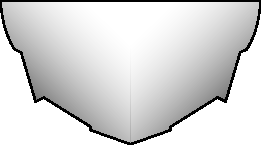
\includegraphics[width=0.34\textwidth]{Images/Design/Hull-shape}
		\label{fig:hull_shape}
	}
	\hfill
	\subfloat[A D-drive inboard motor configuration]{
		
\includegraphics[width=0.34\textwidth]{Images/Design/Motor_config}
		\label{fig:motor_config}
	}
	\caption{Sketch of the hull and motor configuration of Saint Princess}
\end{figure}
This motor and hull was chosen, not because of their properties, but because a boat with this configuration was what the mechanical engineering had available. They also had a catamaran style hull but it was not a motor boat, it was a sail boat and because we need to regulate speed, that would not work. The boat that we got is called Saint Princess, and is a remote controlled yacht. It is specified to go about 30 km/h, it has a water-cooled brushed motor, it also comes with a 8.4 V battery \cite{saint_princess}. That means that this choice of boat lock down the specification of the motor and battery.

\begin{figure}[H]
\centering
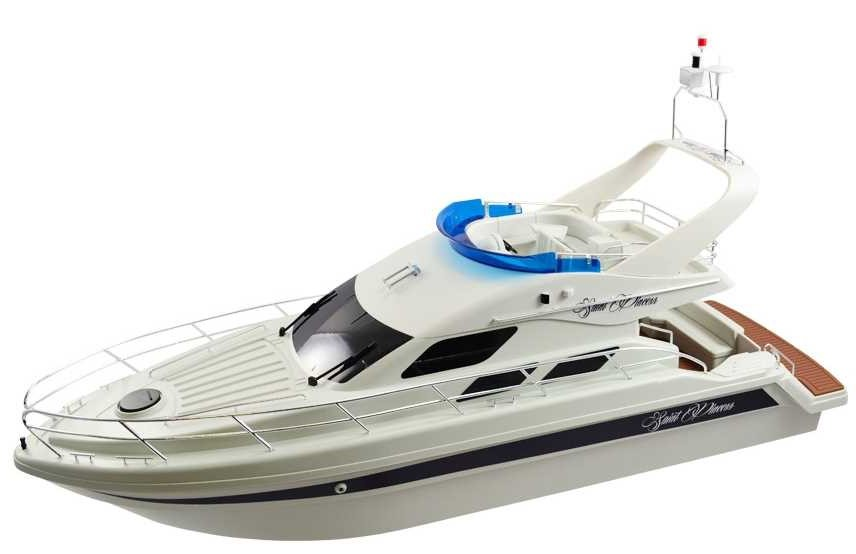
\includegraphics[width=1\linewidth]{Images/Design/saint_princess}
\caption{Saint Princess, a remote controlled yacht\cite{saint_princess}}
\label{fig:saintprincess}
\end{figure}


\subsection{Electronics}
Now with the boat platform figured out, some electronics can be chosen. Micro-computer is needed, to control everything and run our code on. A GPS, and motor controller also needs to be chosen. Lastly when all these things are figured out, then the connections between them needs to be sorted out.

\subsubsection{Micro-computer}
Usually when one wants a micro-computer or system on a chip, it is easy to just choose the Raspberry Pi, since most people know about it. But it made more sense to compare some micro-computers, so a of them were compiled. 

To choose the correct one, some attributes are needed, aswell as some weights for the them. so here is a list of the attributes chosen, what they were weighted; 1 for not important and up to 5 which is every important, and a explanation for the weight.

\begin{description}[itemsep=0mm]
\item[Price] 3. The prince should not be the deciding factor, but 2 equally capable boards, with different prices, the one with the lowest price should come out on top.
\item[Ram] 2. The amount of ram in the system is important when a real time operating system is run on top, but usually this has been considered by the manufacturer.  
\item[Real time operating system] 5. The system requires a real time operating system, since we intend to run 2 different programs on the system at once.
\item[WiFi module] 3. In the architecture a WiFi module is mentioned, still its weight is three because if the board doesn't have it usually an adapter board can be bought, like a USB WiFi adapter.
\item[UART serial] 3. A serial interface is need to talk to a NMEA GPS receiver, but like with WiFi a USB to seraial adapter can be purchased.
\item[SPI] 2. The system does not require SPI to function, but if for some reason a I2C sensors is needed. Or if there is a need for more servos, then it can all be enabled by SPI
\item[PWM] 4. This is required by the system to run the thruster motor, and rudder servo, but if its not there, then I2C or SPI can be used in conjunction with an PWM expansion board.
\item[I2C] 2. This is exactly the same as SPI, if some future sensor needs I2C then it is a nice to have.
\item[Supply voltage] 1. The system isn't really affected by the supply voltage, but a supply around 5 V is a nice to have.
\item[Ethernet Port] 5. This is required by the system to function, if there is no WiFi, then an Ethernet port has to be available to connect to the system 
\item[General purpose I/O] 1. How many I/O's the micro-computer has doesn't really matter, though the more the better.
\item[Support level] 4. This is a subjective measure of how much support it online support a system has. This includes datasheets, forums, etc.
\end{description}

Now that the weight attributes have been figures out, the board to evaluate can be found. There are plenty of them, but the once that ended up being considered are the following:
\begin{itemize}[itemsep=-1mm]
\item Asus Tinter Board \cite{asus-tinker-board}
\item Banana Pi \cite{banana-pi}
\item BeagleBoard X15 \cite{beagle-x15}
\item BeagleBone Black WiFi \cite{beagle-bone}
\item C.H.I.P Pro \cite{chip-pro}
\item Intel Edison \cite{intel-edison}
\item NanoPc-T3 \cite{nanopc}
\item NanoPi 2 Fire \cite{nanopi}
\item Odroid C2 \cite{odroid}
\item OrangePi Plus 2  \cite{orangepi}
\item Parallella \cite{parallella}
\item PineA64+ \cite{pinea64}
\item PixiePro \cite{pixiepro}
\item Raspberry Pi 3B \cite{rpi}
\item Raspberry Pi Zero w \cite{rpi}
\item Udoo Quad \cite{udoo-quad}
\end{itemize}

A comprehensive list of all the micro-computers with all their attributes listed and their final score can be found on table~\ref{tab:board_candidates}. The shows that the board with the best score turns out to be the Raspberry Pi 3B. The Raspberry Pi 3B has wifi built in, an Ethernet port, subjectively a good support level, and the price is also rather low. Another benefit is that the department of engineering already have several of this board in stock.

\begin{figure} [h]
\centering
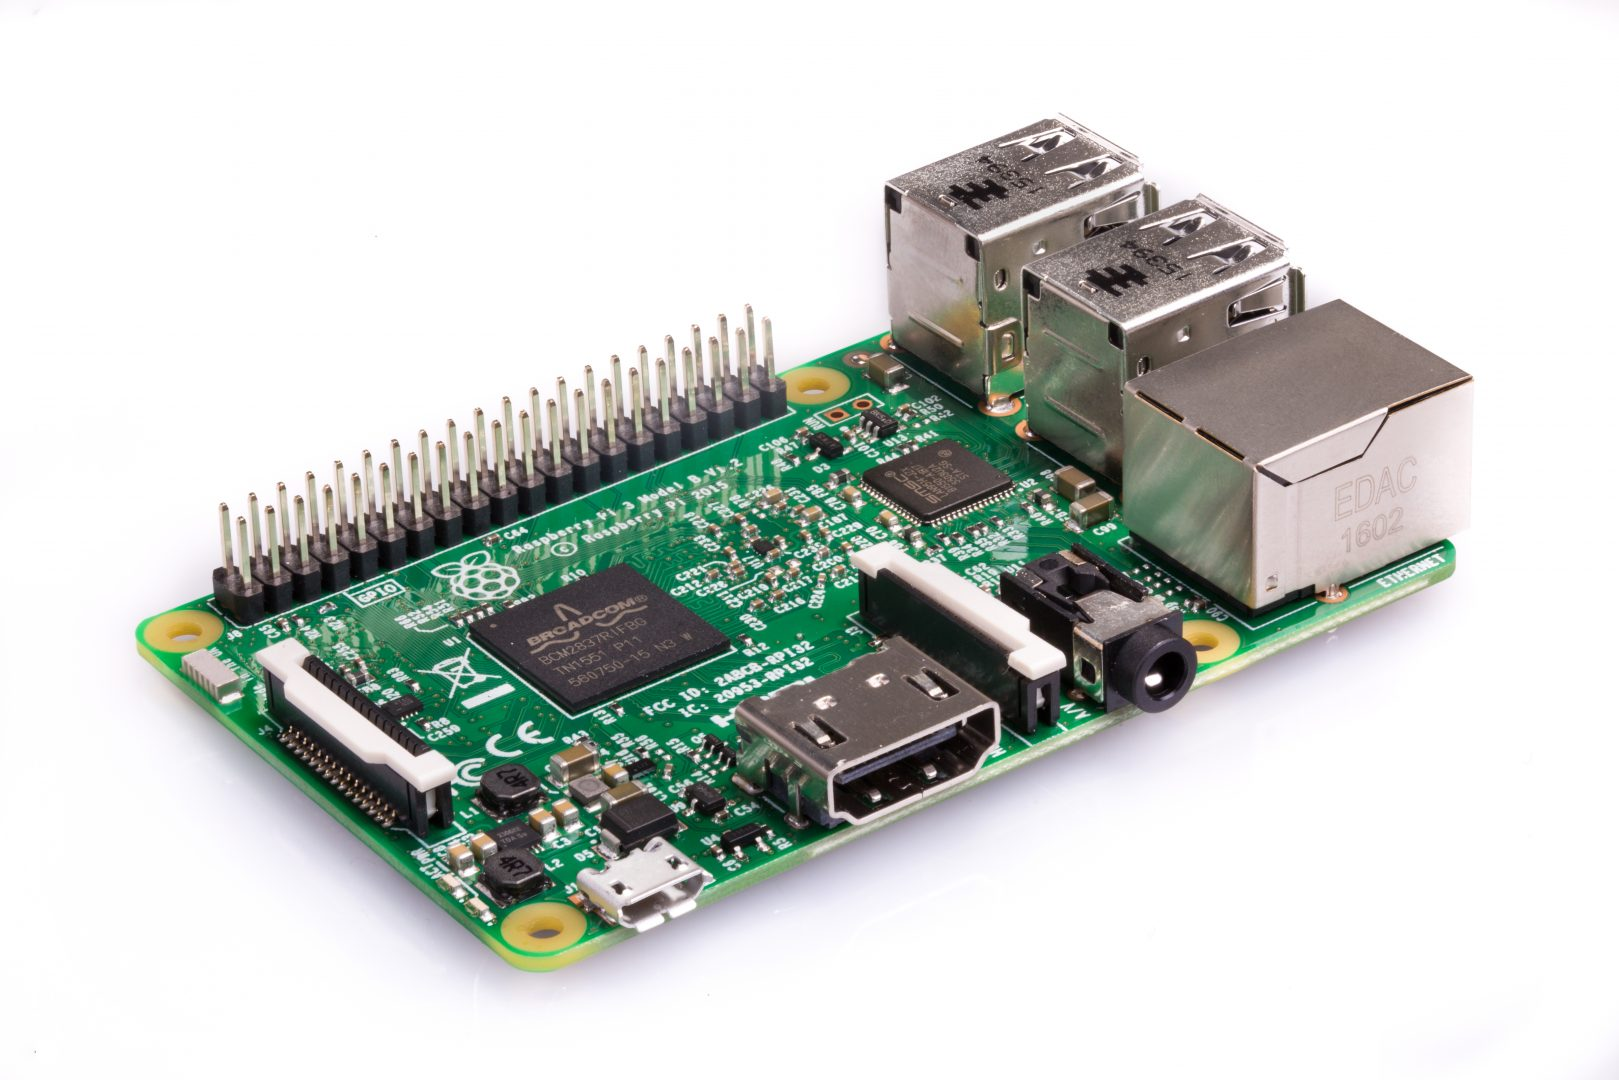
\includegraphics[width=0.7\linewidth]{Images/Design/rpi3b}
\caption{Raspberry Pi 3B}
\label{fig:rpi3b}
\end{figure}


% Table generated by Excel2LaTeX from sheet 'Board_candidates'
\begin{sidewaystable}[htbp]
  \centering
    \begin{tabular}{lrlrrllllllrlrr}
    \toprule
    \textbf{Names} & \multicolumn{1}{l}{\textbf{Score}} & \textbf{Processor} & \multicolumn{1}{l}{\textbf{DKK\footnote{Price is in DKK}}} & \multicolumn{1}{l}{\textbf{RAM}} & \textbf{RTOS} & \textbf{WiFi} & \textbf{UART} & \textbf{SPI} & \textbf{PWM} & \textbf{I2C} & \multicolumn{1}{l}{\textbf{PWR\footnote{Power supply voltage}}} & \textbf{Net\footnote{Ethernet}} & \multicolumn{1}{l}{\textbf{GPIO}} & \multicolumn{1}{l}{\textbf{Support}} \\
    \midrule
    \rowcolor[rgb]{ .851,  .851,  .851} Raspberry Pi 3b & \cellcolor[rgb]{ .388,  .745,  .482}162.0 & 1.2 GHz BCM2837 & 220   & 2048  & \cellcolor[rgb]{ .573,  .816,  .314}Yes & \cellcolor[rgb]{ .573,  .816,  .314}Yes & \cellcolor[rgb]{ .573,  .816,  .314}Yes & \cellcolor[rgb]{ .573,  .816,  .314}Yes & \cellcolor[rgb]{ .573,  .816,  .314}Yes & \cellcolor[rgb]{ .573,  .816,  .314}Yes & 5     & \cellcolor[rgb]{ .573,  .816,  .314}Yes & 40    & 5 \\
    PineA64+ & \cellcolor[rgb]{ .718,  .843,  .502}150.9 & 1.2 GHz ARM A53 & 180   & 2048  & \cellcolor[rgb]{ .573,  .816,  .314}Yes & \cellcolor[rgb]{ .573,  .816,  .314}Yes & \cellcolor[rgb]{ .573,  .816,  .314}Yes & \cellcolor[rgb]{ .573,  .816,  .314}Yes & \cellcolor[rgb]{ .573,  .816,  .314}Yes & \cellcolor[rgb]{ .573,  .816,  .314}Yes & 5     & \cellcolor[rgb]{ .573,  .816,  .314}Yes & 20    & 2 \\
    \rowcolor[rgb]{ .851,  .851,  .851} Asus Tinker Board & \cellcolor[rgb]{ .718,  .843,  .502}150.9 & 1.8 GHz ARM A17 & 440   & 2048  & \cellcolor[rgb]{ .573,  .816,  .314}Yes & \cellcolor[rgb]{ .573,  .816,  .314}Yes & \cellcolor[rgb]{ .573,  .816,  .314}Yes & \cellcolor[rgb]{ .573,  .816,  .314}Yes & \cellcolor[rgb]{ .573,  .816,  .314}Yes & \cellcolor[rgb]{ .573,  .816,  .314}Yes & 5     & \cellcolor[rgb]{ .573,  .816,  .314}Yes & 40    & 3 \\
    BeagleBone Black w & \cellcolor[rgb]{ .812,  .871,  .51}147.7 & 1 GHz ARM A8 & 580   & 512   & \cellcolor[rgb]{ .573,  .816,  .314}Yes & \cellcolor[rgb]{ .573,  .816,  .314}Yes & \cellcolor[rgb]{ .573,  .816,  .314}Yes & \cellcolor[rgb]{ .573,  .816,  .314}Yes & \cellcolor[rgb]{ .573,  .816,  .314}Yes & \cellcolor[rgb]{ .573,  .816,  .314}Yes & 5     & \cellcolor[rgb]{ .573,  .816,  .314}Yes & 92    & 4 \\
    \rowcolor[rgb]{ .851,  .851,  .851} NanoPC-T3 & \cellcolor[rgb]{ .82,  .871,  .51}147.5 & 1.4 GHz ARM A53 & 350   & 2048  & \cellcolor[rgb]{ .573,  .816,  .314}Yes & \cellcolor[rgb]{ .573,  .816,  .314}Yes & \cellcolor[rgb]{ .573,  .816,  .314}Yes & \cellcolor[rgb]{ .573,  .816,  .314}Yes & \cellcolor[rgb]{ .573,  .816,  .314}Yes & \cellcolor[rgb]{ .573,  .816,  .314}Yes & 5     & \cellcolor[rgb]{ .573,  .816,  .314}Yes & 30    & 2 \\
    OrangePi Plus 2 & \cellcolor[rgb]{ .914,  .898,  .514}144.3 & 1.6 GHz ARM A7 & 300   & 2048  & \cellcolor[rgb]{ .573,  .816,  .314}Yes & \cellcolor[rgb]{ .573,  .816,  .314}Yes & \cellcolor[rgb]{ .573,  .816,  .314}Yes & \cellcolor[rgb]{ .573,  .816,  .314}Yes & \cellcolor[rgb]{ .573,  .816,  .314}Yes & \cellcolor[rgb]{ .573,  .816,  .314}Yes & 5     & \cellcolor[rgb]{ .573,  .816,  .314}Yes & 40    & 1 \\
    \rowcolor[rgb]{ .851,  .851,  .851} Raspberry Pi Zero w & \cellcolor[rgb]{ .941,  .906,  .518}143.3 & 1 GHz BCM2835 & 90    & 512   & \cellcolor[rgb]{ .573,  .816,  .314}Yes & \cellcolor[rgb]{ .573,  .816,  .314}Yes & \cellcolor[rgb]{ .573,  .816,  .314}Yes & \cellcolor[rgb]{ .573,  .816,  .314}Yes & \cellcolor[rgb]{ .573,  .816,  .314}Yes & \cellcolor[rgb]{ .573,  .816,  .314}Yes & 5     & No    & 40    & 5 \\
    Banana Pi & \cellcolor[rgb]{ .996,  .922,  .518}141.5 & 1.8 GHz ARM A7-A83T & 810   & 2048  & \cellcolor[rgb]{ .573,  .816,  .314}Yes & \cellcolor[rgb]{ .573,  .816,  .314}Yes & \cellcolor[rgb]{ .573,  .816,  .314}Yes & \cellcolor[rgb]{ .573,  .816,  .314}Yes & \cellcolor[rgb]{ .573,  .816,  .314}Yes & \cellcolor[rgb]{ .573,  .816,  .314}Yes & 5     & \cellcolor[rgb]{ .573,  .816,  .314}Yes & 40    & 1 \\
    \rowcolor[rgb]{ .851,  .851,  .851} Udoo Quad & \cellcolor[rgb]{ .996,  .918,  .514}141.2 & 1 GHz NXP i.MX6Q & 840   & 1024  & \cellcolor[rgb]{ .573,  .816,  .314}Yes & \cellcolor[rgb]{ .573,  .816,  .314}Yes & \cellcolor[rgb]{ .573,  .816,  .314}Yes & \cellcolor[rgb]{ .573,  .816,  .314}Yes & \cellcolor[rgb]{ .573,  .816,  .314}Yes & \cellcolor[rgb]{ .573,  .816,  .314}Yes & 5     & \cellcolor[rgb]{ .573,  .816,  .314}Yes & 76    & 2 \\
    BeagleBoard X15 & \cellcolor[rgb]{ .996,  .914,  .514}140.9 & 1.5 GHz ARM A15 & 1490  & 2048  & \cellcolor[rgb]{ .573,  .816,  .314}Yes & No    & \cellcolor[rgb]{ .573,  .816,  .314}Yes & \cellcolor[rgb]{ .573,  .816,  .314}Yes & \cellcolor[rgb]{ .573,  .816,  .314}Yes & \cellcolor[rgb]{ .573,  .816,  .314}Yes & 12    & \cellcolor[rgb]{ .573,  .816,  .314}Yes & 240   & 4 \\
    \rowcolor[rgb]{ .851,  .851,  .851} NanoPi 2 Fire & \cellcolor[rgb]{ .996,  .851,  .502}136.5 & 1.4 GHz ARM A9 & 140   & 1024  & \cellcolor[rgb]{ .573,  .816,  .314}Yes & No    & \cellcolor[rgb]{ .573,  .816,  .314}Yes & \cellcolor[rgb]{ .573,  .816,  .314}Yes & \cellcolor[rgb]{ .573,  .816,  .314}Yes & \cellcolor[rgb]{ .573,  .816,  .314}Yes & 5     & \cellcolor[rgb]{ .573,  .816,  .314}Yes & 40    & 2 \\
    Intel Edison & \cellcolor[rgb]{ .988,  .757,  .486}129.8 & 0.5 GHz Intel Atom & 570   & 1024  & \cellcolor[rgb]{ .573,  .816,  .314}Yes & \cellcolor[rgb]{ .573,  .816,  .314}Yes & \cellcolor[rgb]{ .573,  .816,  .314}Yes & \cellcolor[rgb]{ .573,  .816,  .314}Yes & \cellcolor[rgb]{ .573,  .816,  .314}Yes & \cellcolor[rgb]{ .573,  .816,  .314}Yes & 5     & No    & 70    & 4 \\
    \rowcolor[rgb]{ .851,  .851,  .851} C.H.I.P. Pro & \cellcolor[rgb]{ .988,  .722,  .478}127.2 & 1 GHz ARM V7-A & 310   & 256   & \cellcolor[rgb]{ .573,  .816,  .314}Yes & \cellcolor[rgb]{ .573,  .816,  .314}Yes & \cellcolor[rgb]{ .573,  .816,  .314}Yes & \cellcolor[rgb]{ .573,  .816,  .314}Yes & \cellcolor[rgb]{ .573,  .816,  .314}Yes & \cellcolor[rgb]{ .573,  .816,  .314}Yes & 5     & No    & 27    & 4 \\
    Odroid C2 & \cellcolor[rgb]{ .976,  .518,  .439}112.5 & 1.5 GHz ARM V8 & 290   & 2048  & \cellcolor[rgb]{ .573,  .816,  .314}Yes & No    & \cellcolor[rgb]{ .573,  .816,  .314}Yes & No    & No    & \cellcolor[rgb]{ .573,  .816,  .314}Yes & 5     & \cellcolor[rgb]{ .573,  .816,  .314}Yes & 40    & 2 \\
    \rowcolor[rgb]{ .851,  .851,  .851} Parallella & \cellcolor[rgb]{ .976,  .514,  .439}112.4 & 0.8 GHz ARM A9 & 1000  & 1024  & \cellcolor[rgb]{ .573,  .816,  .314}Yes & No    & \cellcolor[rgb]{ .573,  .816,  .314}Yes & \cellcolor[rgb]{ .573,  .816,  .314}Yes & ?     & \cellcolor[rgb]{ .573,  .816,  .314}Yes & 5     & \cellcolor[rgb]{ .573,  .816,  .314}Yes & 48    & 2 \\
    PixiePro & \cellcolor[rgb]{ .973,  .412,  .42}104.9 & 1 GHz .iMX6Q  & 810   & 2048  & \cellcolor[rgb]{ .573,  .816,  .314}Yes & \cellcolor[rgb]{ .573,  .816,  .314}Yes & \cellcolor[rgb]{ .573,  .816,  .314}Yes & \cellcolor[rgb]{ .573,  .816,  .314}Yes & ?     & \cellcolor[rgb]{ .573,  .816,  .314}Yes & 5     & No    & 10    & 1 \\
    \bottomrule
    \end{tabular}%
  \caption{A weighted comparison of micro-computers.}
  \label{tab:board_candidates}%
\end{sidewaystable}%


\subsubsection{GPS}
Choosing a GPS receiver is a challenge, because the most important attribute is the precision of position data it can supply. Regular GPS receivers like the one most phones and car GPS navigations systems have a precision of about 5 meters. There Exist receivers that are sub meter precision, and even once that can supply a position with a accuracy down in the centimeter range. 
For this system, the higher the accuracy the better, but this is just a question of cost. 

Because the only factor in choosing a GPS basically is cost, then i make sens to use what ever is already available at the department of engineering, and in stock was a u-blox NEO-7M-0-000 \cite{ublox-datasheet}. 
\begin{figure}[H]
\centering
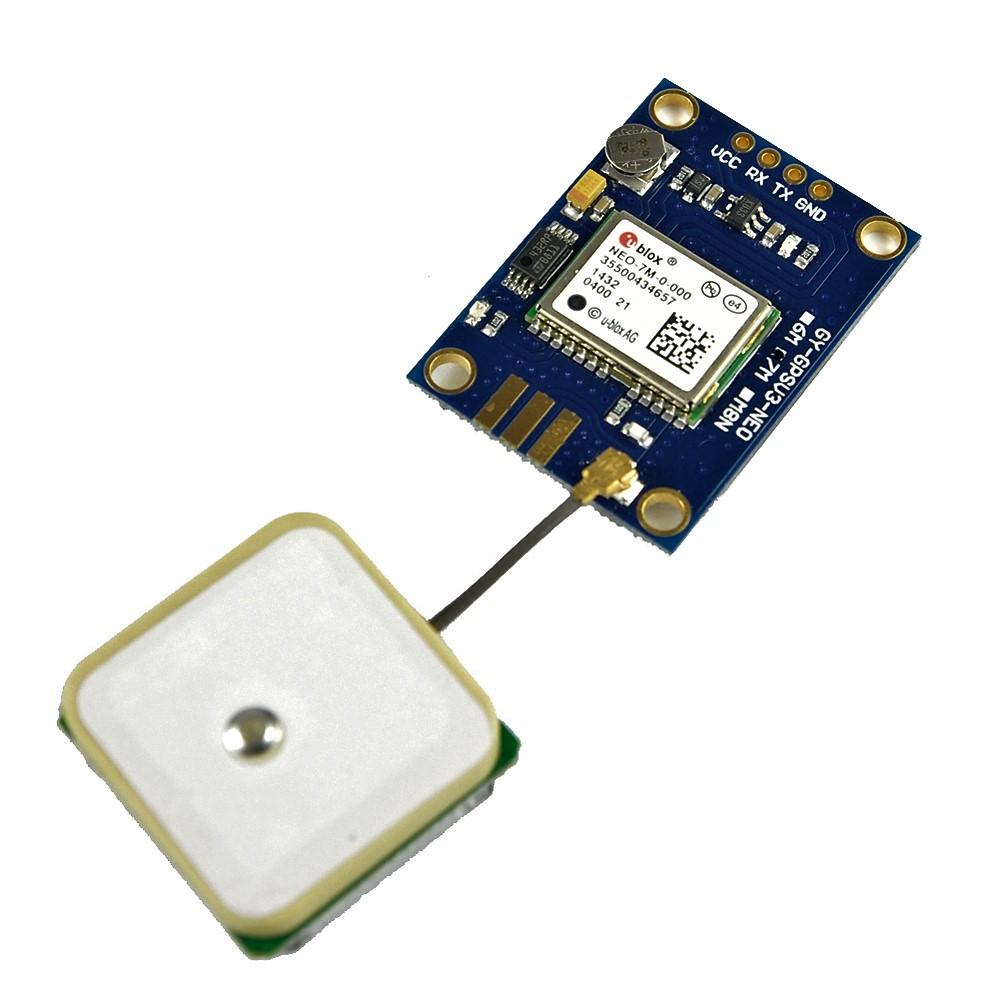
\includegraphics[width=0.5\linewidth]{Images/Design/ublox}
\caption{ublox NEO-7M-0-000 with antenna\cite{ublox-image}}
\label{fig:ublox}
\end{figure}
Attributes to consider with the NEO-7M receiver is the horizontal position accuracy which a absolute maximum of 2.5 meters. It has a cold-start time of 30 seconds, meaning that it takes up to 30 seconds before it receives fix from enough satellites to get a position. It a heading accuracy of 0.5 degrees, and a velocity accuracy of 0.1 m/s. 

\subsubsection{Motor controller}
The choice of motor controller is bound by the motor that comes with Saint Princess, and this motor is proprietary so there is no way to get the actual specification of it. Therefore measurements on the motor have been conducted, as seen on figure~\ref{fig:motoramperagetest}. The highest amperage draw under load was measured to be 29 A, So a motor controller that can handle this has to be found.

\begin{figure}[H]
\centering
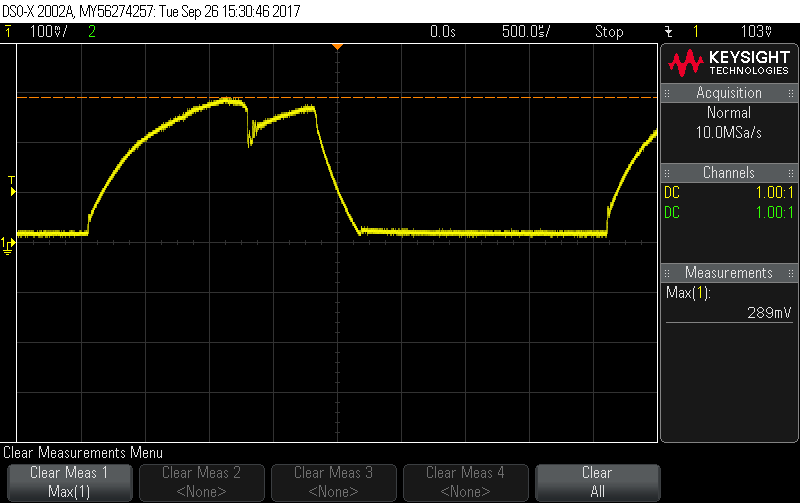
\includegraphics[width=0.7\linewidth]{Images/Design/motor_amperage_test}
\caption{Amperage measurement, short duration loaded by water. 10mV : 1A}
\label{fig:motoramperagetest}
\end{figure}

Cytron MD30C rev. 2\cite{md30}, is a brushed motor controller, what can handle 30 ampere continuously, and up to 80 amperes for up to a second. It also has a built in PWM generator, where the frequency can be controlled by either an internal or and external potentiometer. In this system the micro-computer generates the PWM, and it can also be set up to handle that, ei. an external PWM signal.

\begin{figure}[H]
\centering
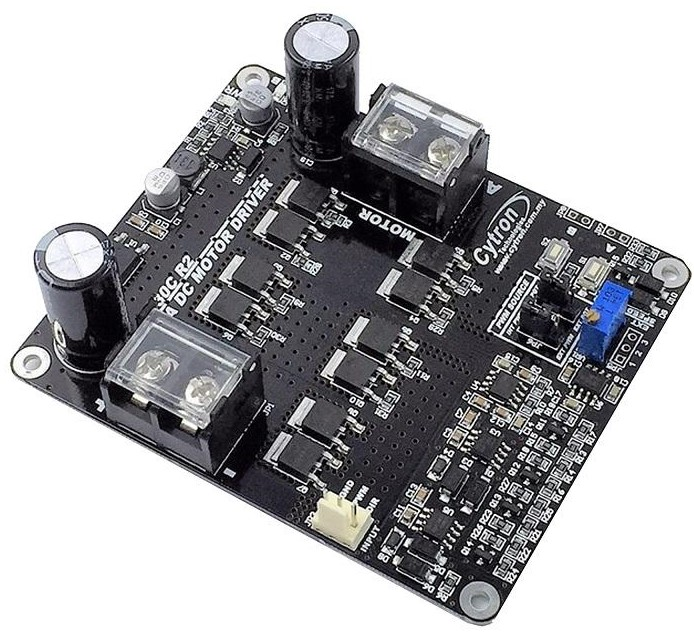
\includegraphics[width=0.7\linewidth]{Images/Design/cytron}
\caption{Cytron MD30C rev. 2, motor controller}
\label{fig:cytron}
\end{figure}

\subsubsection{Connections}
Now that all the components have been picked out, they need to be put together. 
A battery of 8.4 V, is to high voltage for the Raspberry pi and the rudder servo. Therefore a step down circuit is needed, and just to make sure that the servo doesn't introduce a lot of noise in the supply to Raspberry pi, it should get its own step down. both step downs need to be able go down to 5 V. Once again the department of engineering had some in stock, the ones they got were LM2596 as seen on figure~\ref{fig:stepdown} \cite{stepdown}. The LM2596 can deliver up to 2 amperes with out a heat sink, this enough for the raspberry pi, and it is reasonable to think that a servo in Saint Princess is not going to draw more then 2 amperes.
\begin{figure}[H]
\centering
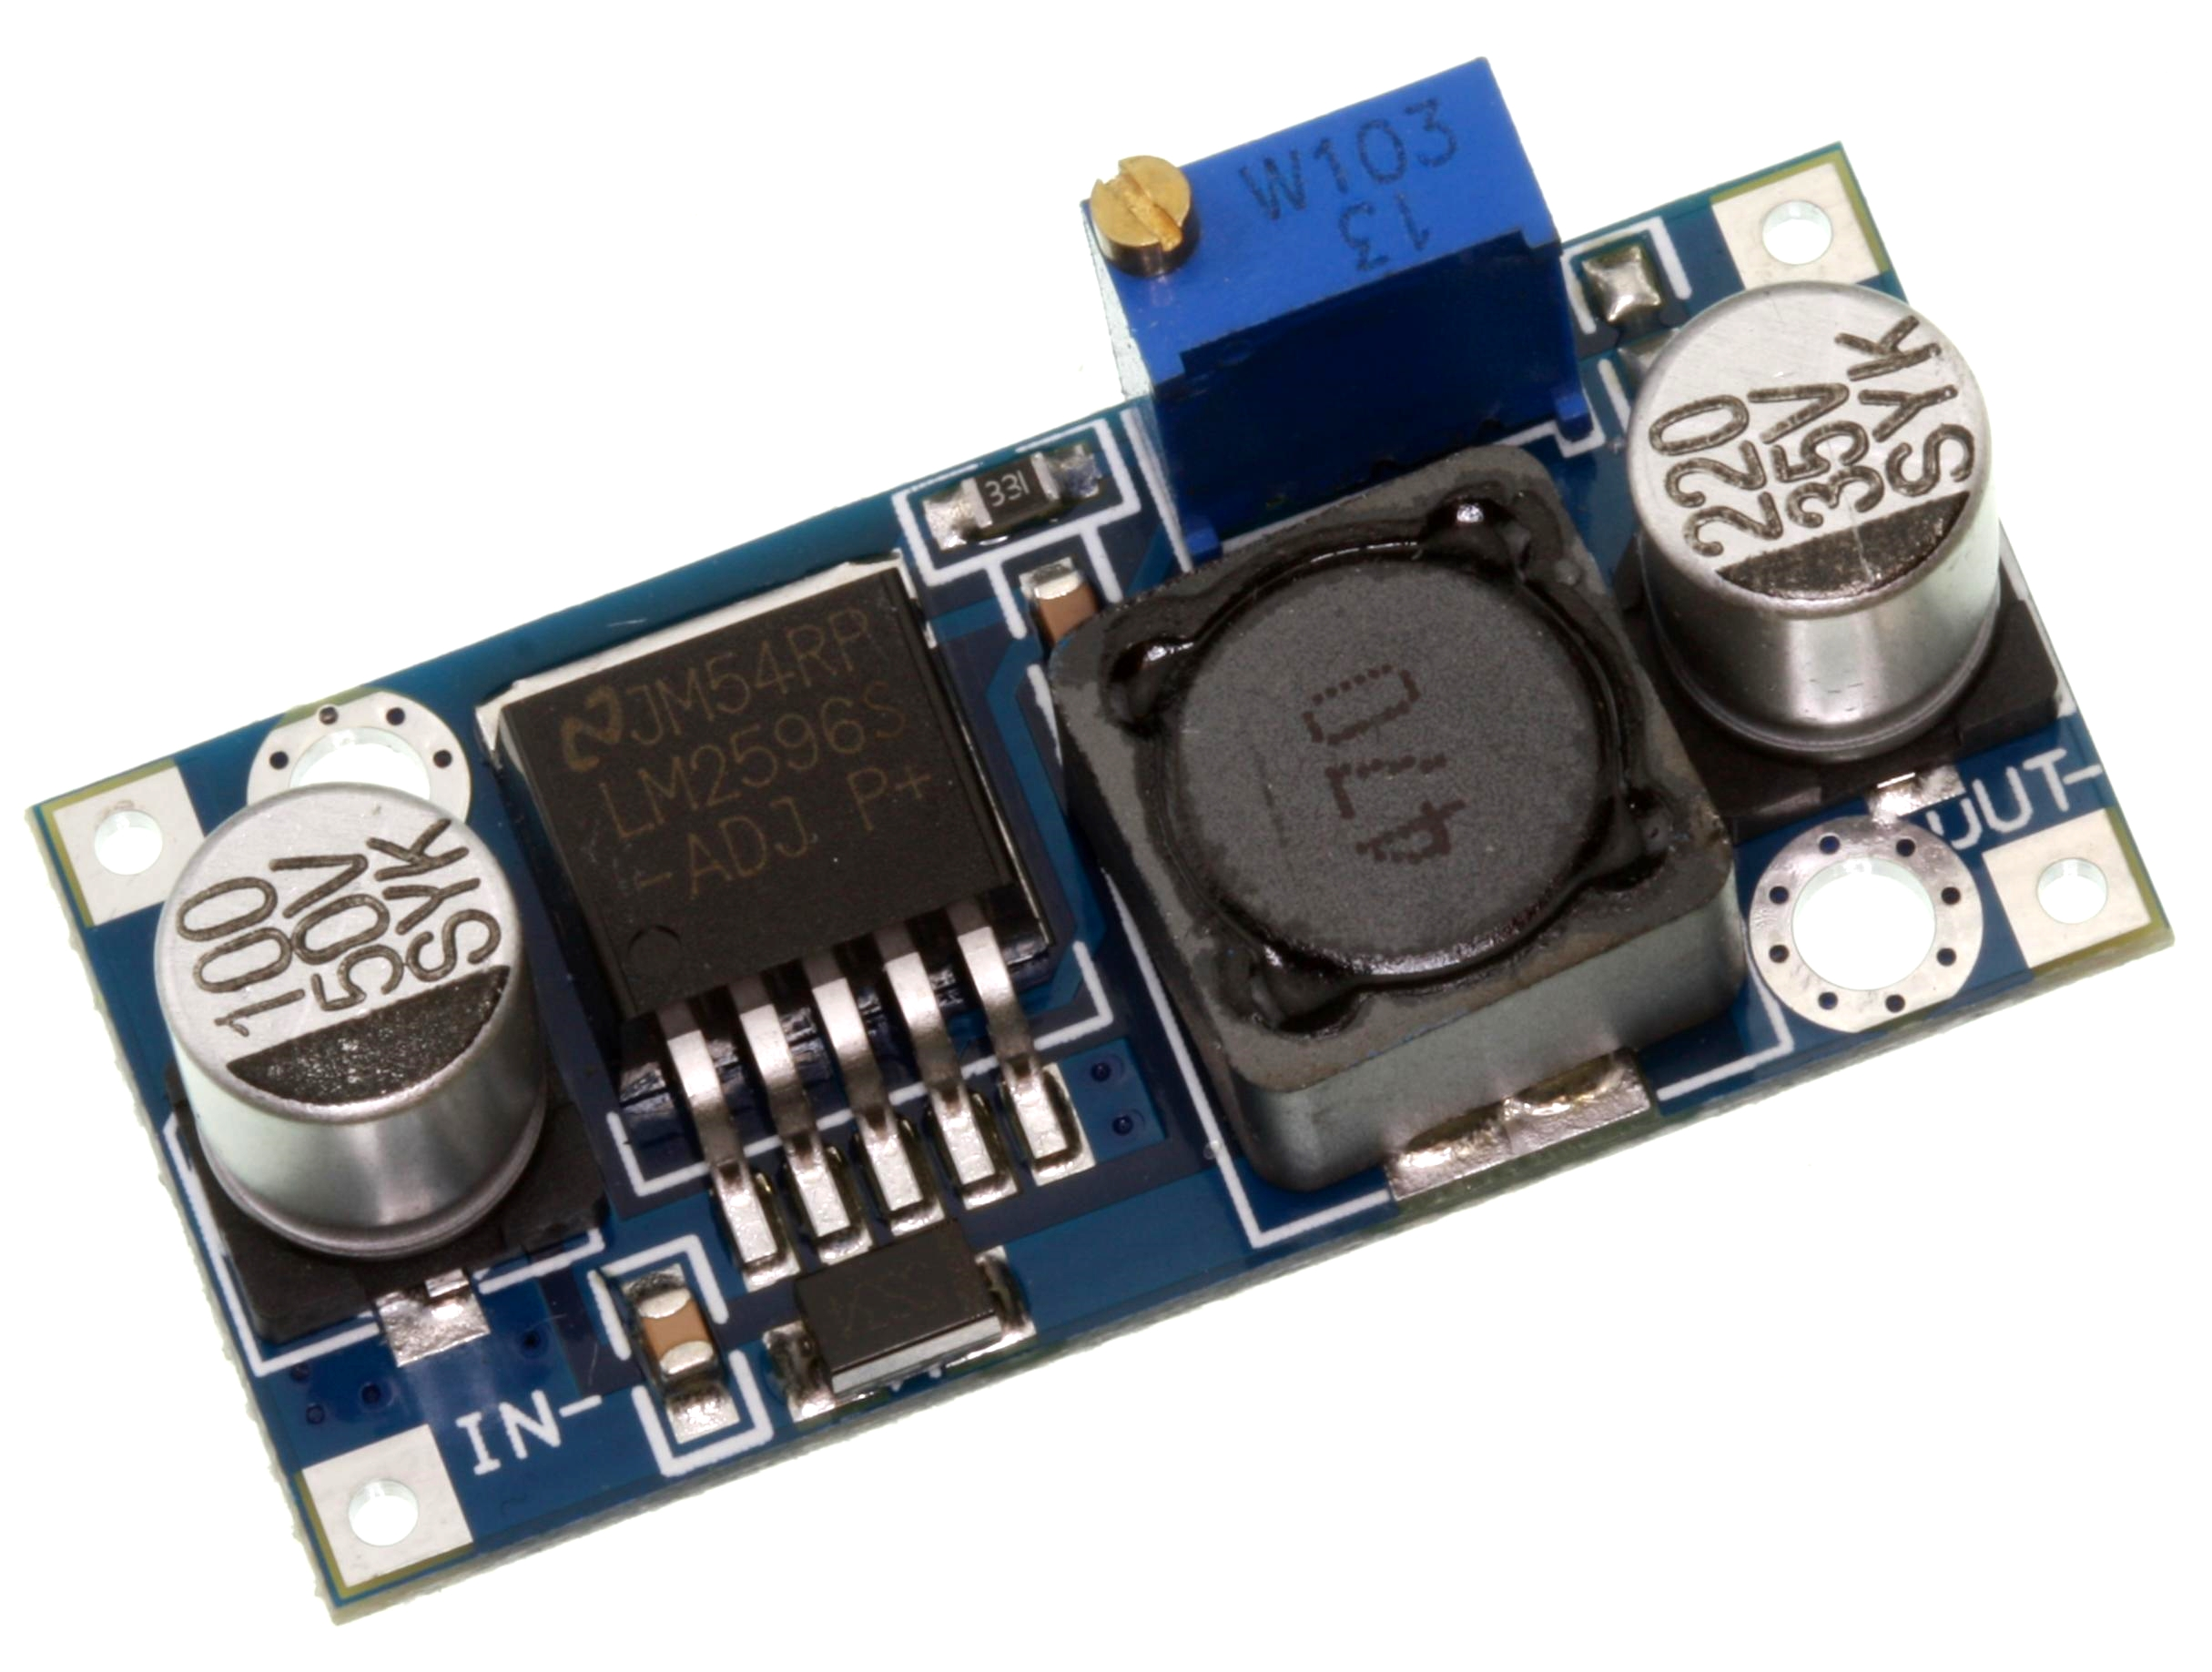
\includegraphics[width=0.4\linewidth]{Images/Design/stepdown}
\caption{LM2596 breakout}
\label{fig:stepdown}
\end{figure}

There is one last problem to sort out, and that is the raspberry pi output is 3.3 V. This is fine for the motor controller PWM, since the motor controller, just need a logic level high of either 5 V or 3.3 V. But for the servo, a 5 V logic level high is need for the PWM. Therefore a level shifter is needed the one that the department of engineering has is the one depicted in figure~\ref{fig:levelshifter} \cite{levelshifter}. It can convert from 5 V to 3.3 V or the other way around. 

\begin{figure}[H]
\centering
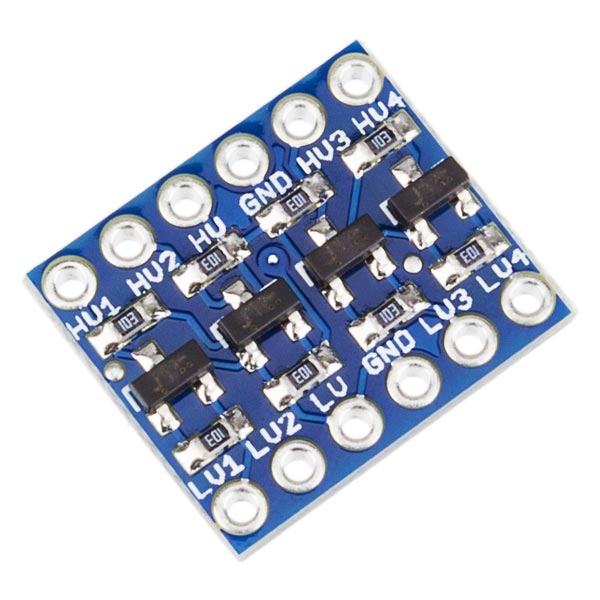
\includegraphics[width=0.3\linewidth]{Images/Design/levelshifter}
\caption{LM2596 breakout}
\label{fig:levelshifter}
\end{figure}

Now that all the components have been specified, the hardware design can be drawn as seen on~\ref{fig:hardware_design}. On the figure it can be seen how the battery is split in to the 2 step downs and the motor controller uses the 8.4 V directly. Also how the Raspberry pi is connected to the servo through the level shifter.

\begin{figure}[H]
\centering
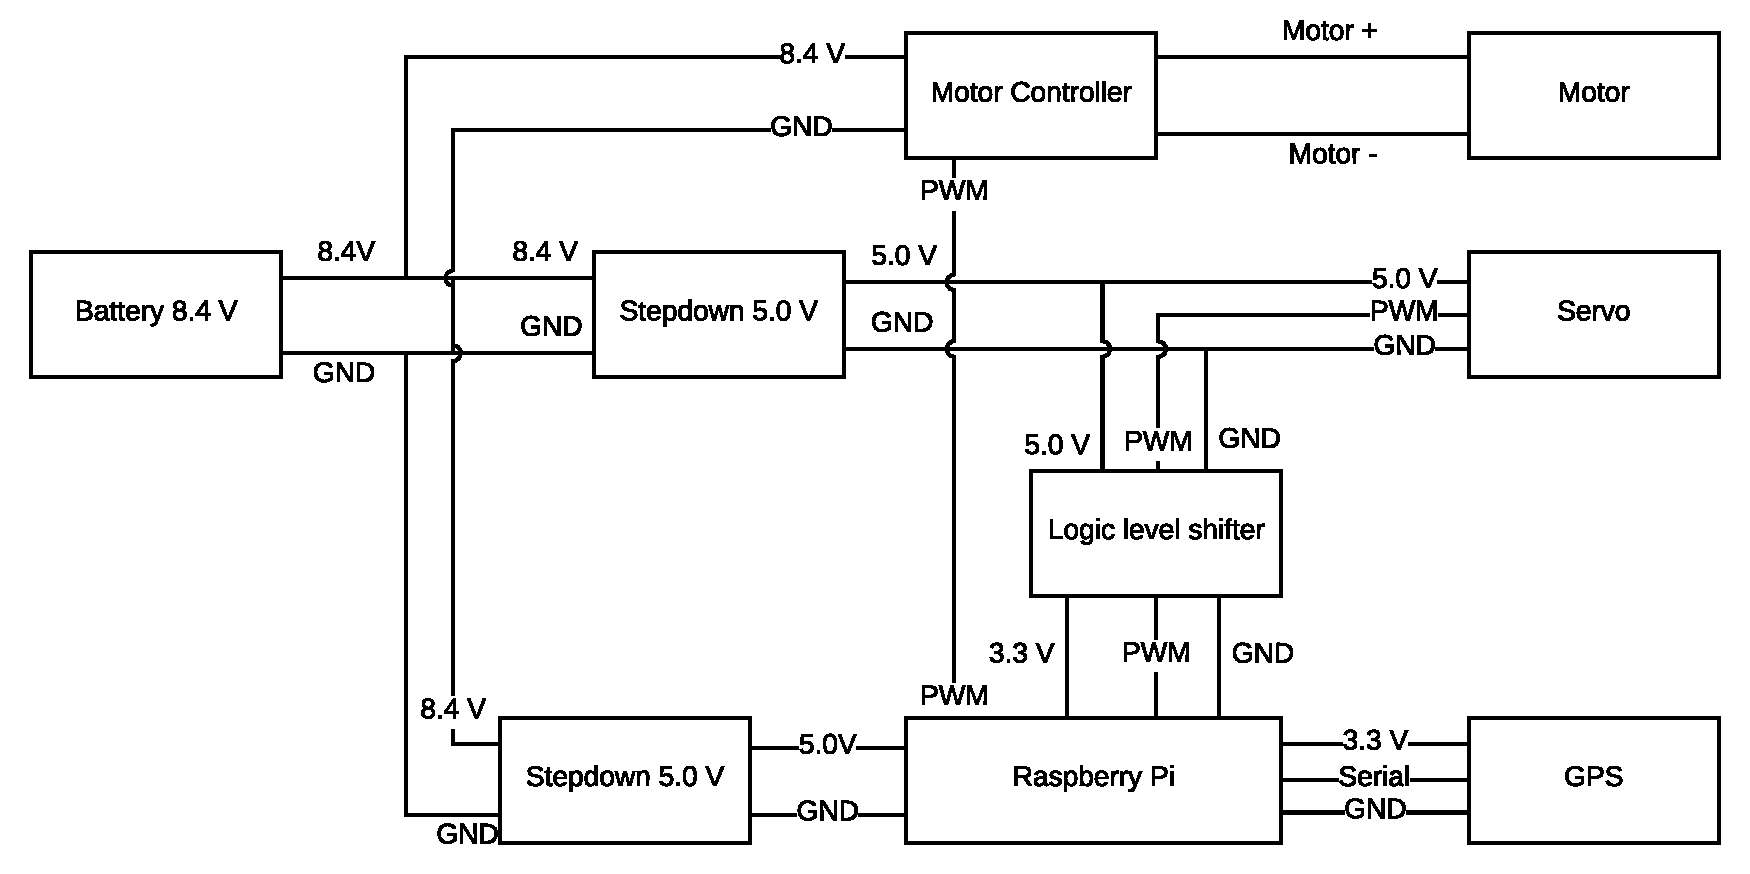
\includegraphics[width=1\linewidth]{Images/Design/Hardware_design}
\caption{Hardware design}
\label{fig:hardware_design}
\end{figure}


% Boat
% 
%Component choises
%	Realtime operating system
%	Motor
%	Servo
%	Motor Controller
%	Battery
%	Regulator
%	GPS
%	Logic level shifter